\chapter{Introduction}
\label{chp:introduction}


%%%%%%%%%%%%%%%%%%%%%%%%%%%%%%%%%%%%%%%%%%%%%%%%%%%%%%%%%%%%%%%%%%%%%%%
\section{Background}
\label{sec:background}

Autonomous cars have the potential to revolutionize transportation by providing mobility to a broad range of people. 
They will increase the independence of people incapable of driving, reduce the number of road accidents caused by driver negligence, and reduce both road congestion and pollution by optimising routes and driving style, to name just a few ways in which autonomous cars are expected to impact our daily lives \cite{klaver}. 
However, there are numerous challenges to large scale deployment of road-going autonomous cars. 
Public roads are an unpredictable environment, and autonomous cars face a wide variety of scenarios which are difficult to program for; 
there are many edge cases which will require the vehicle to not only respond quickly, but also operate at its handling limits to avoid collisions and ensure the safety of its occupants \cite{Barab_s_2017}.

\subsection{Autonomous racing}
The increasing popularity of autonomous vehicles, along with the need to build driving software robust enough to handle these edge cases has led to the emergence of autonomous racing as a new research field. 
Racing leagues such as F1tenth and Indy Autonomous challenge, who's vehicles are shown in Figure \ref{fig:f1tenth_car} and \ref{fig:iac_car} respectively, provide a safe and controlled environment for teams to design and improve driving software with a clear evaluation metric in mind: achieving the fastest lap time navigating around a track \cite{Betz2021}. 
This necessitates the vehicle travelling at high speeds and accelerations, and close to the friction limits of its wheels.
To safely navigate the vehicle under these conditions, the driving software must perform the challenging task of planning optimal trajectories in highly dynamic and uncertain environments, whilst generating precise control commands at high frequencies to ensure this trajectory is executed.
Autonomous racing has led to novel ideas which may directly lead to breakthroughs in safe production driverless car technology, especially in those edge cases where cars must operate close to their handling limits to avoid collisions.
Because the major difference between road going autonomous car and racing problems is the speed of operation \cite{Wadekar2021}, racing can be seen as a proxy for the production car edge case. 
The argument is that if a driving software works in the extreme racing scenario, then similar design principles can be followed to build driving software for the road-going case \cite{Weiss2020a}.

\begin{figure}
\centering
\begin{minipage}{.5\textwidth}
  \centering
  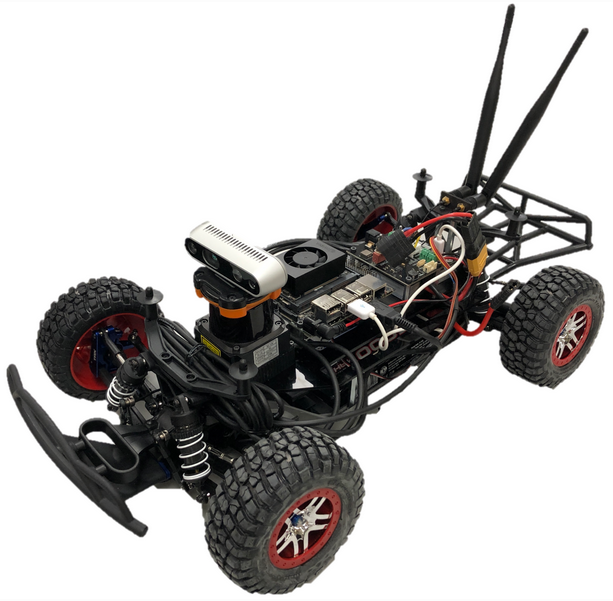
\includegraphics[height=.6\linewidth]{contents/chapt1/figs/f1tenth_car.png}
  \captionof{figure}[The F1tenth standard racecar]{The F1tenth standard \\racecar.}
  %[F1tenth standard racecar]{The F1tenth standard racecar}
  \label{fig:f1tenth_car}
\end{minipage}%
\begin{minipage}{.5\textwidth}
  \centering
  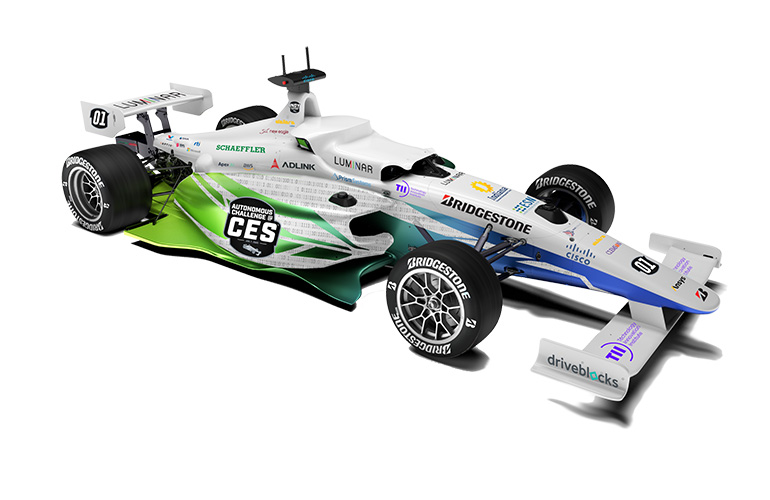
\includegraphics[height=.6\linewidth]{contents/chapt1/figs/indy_auto_car.jpg}
  \captionof{figure}[The Indy Autonomous challenge official racecar]{Dallara AV-21, the Indy Autonomous challenge official racecar.}
  %\caption[Indy Autonomous challenge official racecar]{Dallara AV-21, the Indy Autonomous challenge official racecar}
  \label{fig:iac_car}
\end{minipage}
\end{figure}


\subsection{Challenges to developing autonomous racing software}
\label{sec:auto_race_challenges}
Driving software is typically first developed and tested in simulation before being deployed onto physical vehicles.
This deployment onto physical vehicles presents a major challenge, known as the `sim2real' gap, due to discrepancies between the simulated and actual vehicle models used for planning. 
These discrepancies almost always exist because it is difficult to measure the parameters of the dynamic model precisely \cite{Hewing2018}. For instance, the tyre friction coefficient at every point along the track is not only a function of track roughness, but also tyre and track temperature, and tyre degradation; all of which vary during the race \cite{Sharp2016}.
These discrepancies can cause the physical vehicle to deviate from its planned path, leading to catastrophic failure in some circumstances.
Because the discrepancies also pertain to the handling limit of the vehicle, their effect is more catastrophic when the vehicle is operating at its handling limits, as in the racing scenario \cite{Hewing2018}. 
For instance, if the vehicle is operated close to the estimated friction limit of its tyres, but the actual friction limit is lower than expected, then the vehicle risks losing control.
As such, it is pertinent that any driving software for racing applications should be robust to model inaccuracies.
The development of driving software for racing that is robust to model inaccuracies near the vehicle handling limits will benefit production vehicles by providing solutions to handle edge cases effectively.

\subsection{Current approaches to autonomous driving software}
Current research in developing autonomous racing software architectures fall into one of two broad categories: the classic and end-to-end approach.
The classic approaches decouples the racing problem into perception, planning and control \cite{Fuchs2021}, as shown in Figure \ref{fig:architecture_comparison} (a). 
Perception algorithms derive knowledge about the vehicles surroundings. 
This includes constructing a map, localising the vehicle, and detecting objects. 
The function of trajectory planning is to compute a minimum time trajectory through this map, consisting of a path ($x$ and $y$ coordinates) and velocity. Controllers then compute actuator commands that minimise the error between the actual and planned trajectory which facilitates the deployment of driving software onto physical vehicles \cite{Betz2021}. 
Classical approaches have achieved impressive results owing to the use of optimisation techniques for planning and control. 
However, there are limitations to these optimisation techniques, such as the requirement for expensive computation (especially for non-linear dynamic models), expensive sensor suites due to the need for frequent and accurate state information, and lack of flexibility in the cost function. 
In particular, reliance on an accurate vehicle dynamics model is a serious issue due to the difficulty of measuring the model parameters \cite{Kabzan2019, Pan2017}.

\begin{figure}[!htb]
\centering
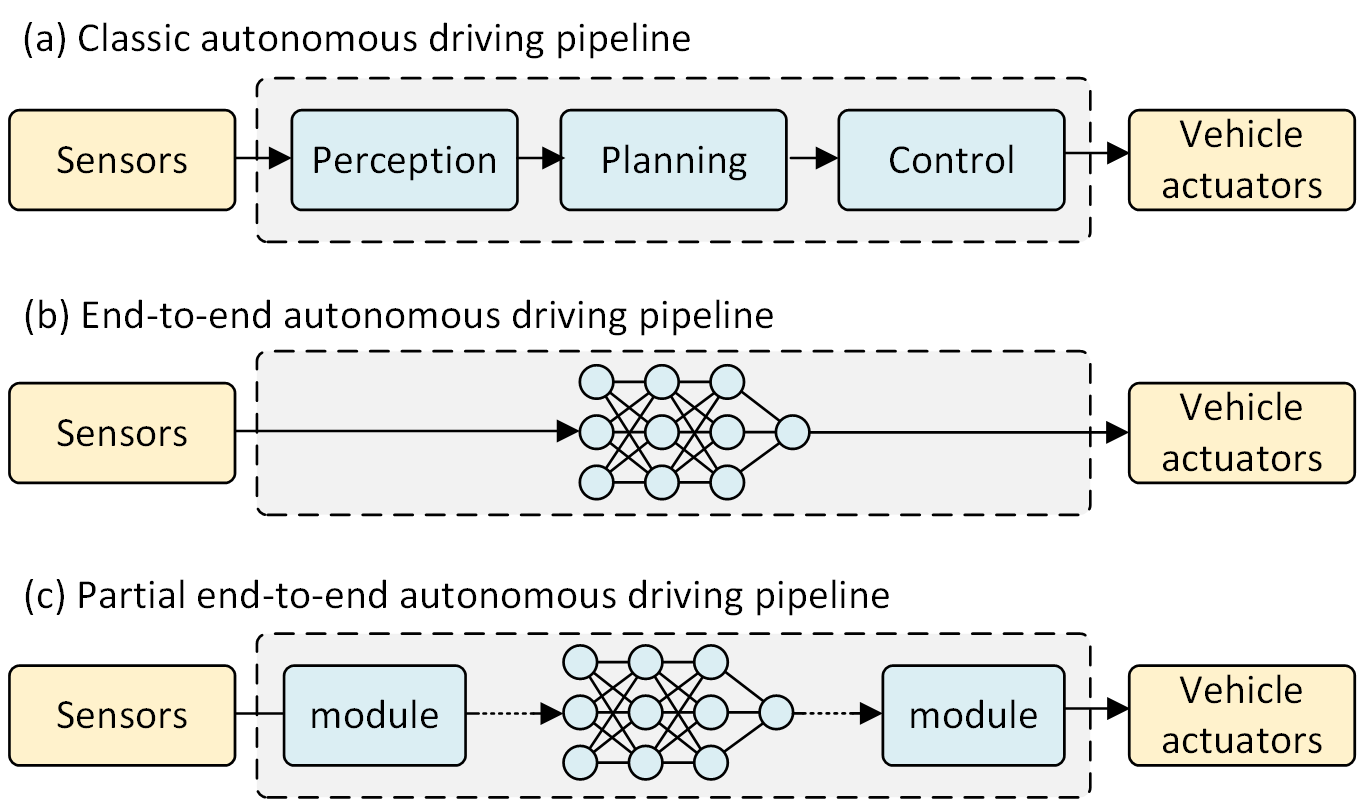
\includegraphics[width=\textwidth*8/10]{contents/chapt1/figs/architecture_comparisons.png}
\caption[A comparison of the commonly used driving software architectures]{A comparison of the commonly used driving software architectures.}
\label{fig:architecture_comparison}
\end{figure}

The limitations of classical methods has led to research in learning-based systems that improve the vehicle dynamics model or action policy with real-world data and allow more complex cost formulations and non-linear dynamics \cite{Fuchs2021}.
Many learning approaches use an end-to-end pipeline, illustrated in Figure \ref{fig:architecture_comparison} (b), whereby a single neural network predicts control outputs from sensor data \cite{Betz2021}.
The neural networks used in end-to-end approaches are typically trained using imitation or reinforcement learning paradigms.
Imitation learned neural networks are trained to mimic an expert such as a human or optimisation method.
This is particularly useful when the neural network has access to lower cost sensors, allowing the optimisation method policy to be executed on a cheaper sensor suit \cite{Pan2017}. 
Neural networks trained with imitation learning have also shown greater robustness to sensor failure and faster online execution time \cite{Wadekar2021} than expert optimisation methods \cite{Lee2019}. 
However, imitation learning is not a suitable method for training a neural network policy in scenarios where expert training data is not available, as in cases where optimisation methods fail \cite{Fuchs2021a}.

%Reinforcement learning
Reinforcement learning optimises a neural network policy to maximise a scalar reward signal through direct interaction with the environment \cite{Plaat_2022}. 
The benefit of using reinforcement learned neural networks are similar to the imitation learning approach, i.e., less stringent sensor requirements, robustness to sensor failure, and fast online execution time. However, the technique allows for more complex cost formulation and negates the need for expert training data \cite{Fuchs2021}.
The approach has shown state of the art results in both time trail and multi-agent settings \cite{Song2021}.
However promising the results from approaches utilising the end-to-end pipeline are, most applications are still limited to simulation.
There is difficulty in deploying end-to-end systems due to the degradation in performance caused by vehicle model inaccuracies \cite{Ivanov2020}, as discussed in Section \ref{sec:auto_race_challenges}. 
These difficulties are usually overcome by retraining the neural network policy on the physical vehicle after deployment, which is an inherently risky process, as retraining the policy network requires exploration which may result in the vehicle crashing \cite{Chisari2021}.
Furthermore, neural network behaviour is difficult to interpret, especially where the neural network takes the place of the entire driving pipeline \cite{Evans2021}.


A relatively unexplored possibility to address issues from the end-to-end approach is to synthesise the classic and end-to-end pipelines by modifying a section of the classic pipeline with a neural network, as shown in Figure \ref{fig:architecture_comparison}. 
This is known as a partial end-to-end pipeline \cite{Betz2021}. 
In particular, a promising approach to address the degradation in performance of end-to-end systems due to model inaccuracies is to use a neural network for trajectory prediction, in conjunction with a set of controllers for trajectory tracking \cite{Capo2020}.
This approach benefits from the advantages of learning-based end-to-end systems, i.e., complex cost formulation, fast online computation and learning from real-world data, while also leveraging the reliability of the hierarchical structure from the classical approach \cite{Ghignone2022}. 


\section{Project objectives and scope}
\label{sec:objectives}

Our goal is to investigate and develop a partial end-to-end driving autonomous driving software architecture as a method to address issues with typical learning, i.e. end-to-end approaches, with specific reference to robustness to inaccuracies in the vehicle model. Therefore, the objective of the project is two-fold:

\begin{enumerate}
  \item Develop a framework for partial end-to-end autonomous racing software
  \item Benchmark the partial end-to-end framework against end-to-end techniques with and without model discrepancies
\end{enumerate}

We do so within a simulated F1Tenth racing simulation environment. 
This platform is easily extended to real-world vehicles, allowing for the easy extension of future work on the topic.
The autonomous driving software is developed to achieve the goals of navigating the vehicle around the track while minimising lap time and number of collisions. 
The exact scenario we solve for is a time trial, whereby there is only one vehicle on the track at a time. Furthermore, we make the assumption that the track dimensions are perfectly known. 
Finally, we choose to limit the scope of the project by only developing reinforcement learning techniques for training to negate the requirement for expert training data.


\section{Document outline}
\label{sec:outline}

Chapter \ref{chp:litreview} constitutes an overview of the existing approaches to solving the autonomous racing problem in literature. 
We briefly discuss solutions from the classic pipeline and end-to-end pipelines, before reviewing partial end-to-end approaches. 
The core concepts of Markov decision processes reinforcement learning are then discussed in Chapter \ref{chp:reinforcement_learning}.
This is followed by a description of the simulation setup for the racing environment in Chapter \ref{chp:simulation}.
Our partial end-to-end system design is detailed in Chapter \ref{chp:design}, followed by experiments and results in Chapter \ref{chp:experiments}. 
We conclude with a summary of our findings and proposal for future work in Chapter \ref{chp:conclusion}.